Este fue un estudio doble-ciego, monocéntrico de grupos paralelos, placebo-controlado; y fue llevado a cabo en su totalidad en la Subdirección de Investigaciones Clínicas del Instituto Nacional de Psiquiatría Ramón de la Fuente Muñiz (INPRFM) en la Ciudad de México.
La investigación forma parte de un proyceto mayor financiado por CONACYT:
``Cambios en la estructura y conectividad funcional cerebrales relacionados a la mejoría clínica en pacientes con adicción a la cocaína después de un tratamiento con esitmulación magnética transcraneal'',
clave S0008-2015-2-260971, bajo la dirección del doctor Eduardo Garza Villarreal y aprobado por el Comité de Ética del INPFRM (CEI/C/070/2016).

\section{Muestra}
Tanto pacientes de la clínica de adicciones del INPFRM como externos que cumplieran con el diagnóstico de dependencia de cocaína (F14.2x) del DSM 5 \parencite{APA2015} fueron reclutados para participar en el ensayo clínico.\par
XXX sujetos fueron asignados aleatoriamente a los distintos grupos de estimulación.
Un grupo recibió estimulación sobre la corteza prefrontal dorsolateral izquierda y el otro, el protocolo sham de estimulación simulada sobre la misma área.
Una muestra de sujetos controles sanos pareados por edad, sexo y nivel de educación fue extraída de los datos de un estudio realizado con anterioridad en el INPFRM \parencite{Garza2017}.

\section{Criteros de selección}
Se siguieron los criterios de selección establecidos en el proyecto principal.
Estos fueron propuestos con la intención de disminuir la posibilidad de aparición de cualquier variable extraña y de seguir los lineamientos de seguridad tanto para la resonancia magnética como la estimulación magnética transcraneal.

\subsection{Criterios de inclusión}
Todos los participantes debían cumplir con los siguientes criterios para ser registrados en el estudio y ser asignados a uno de los grupos de investigación:
\begin{itemize}
    \item Tener una edad mínima de 18 años y máxima de 50 años.
    \item Ser usuario de cocaína durante al menos 2 años, con un uso promedio actual mínimo de 3 veces a la semana y periodos de abstinencia contínua menores a un mes durante el último año.
    \item Poseer un nivel de lectura de al menos 6to año de primaria.
    \item Tener la capacidad de dar un consentimiento informado válido.
    \item Ser diestro.
    \item Tener un índice de masa corporal menor o igual a 30.
    \item Para las participantes del sexo femenino y en edad fértil; comprometerse a utilizar una forma médicamente aceptable\footnote{Métodos aceptables fueron: píldora anticonceptiva, preparación hormonal, DIU o depósito (anillo, inyección, implante) y/o algún método anticonceptivo de barrera (diafragma, esponja, espermicida o condón).} de anticonceptivo y no quedar embarazada durante el estudio.
\end{itemize}

\subsection{Criterios de exclusión}
Los participantes fueron excluidos del estudio si presentaron cualquiera de las siguientes características:
\begin{itemize}
    \item Antecedentes personales o familiartes de primer grado de cualquier trastorno neurológico, historia personal de neurocirugías previas o traumas craneoencefálicos que hayan producido pérdida de la conciencia.
    \item Tener alguno de los siguientes: marcapasos cardiáco, estimuladores neuronales, desfibriladores implantable, bomba de medicación implantada, líneas intracardiacas, implantes intracraneales (clips de aneurisma, derivaciones, estimuladores, implantes cocleares o electrodos) o cualquier objeto metálido dentro o cerca de la cabeza que no pueda ser retirado de forma segura.
    \item Esquirlas de metal o proyectiles metálicos en la cabeza o cuerpo.
    \item Uso actual de cualquier droga de investigación o de cualquier medicamento con acción proconvulsivante\footnote{Antidepresivos tricíclicos o neurolépticos que disminuyen el umbral convulsivo.}.
    \item Presión intracraneal aumentada.
    \item Historia de esquizofrenia, trastorno bipolar, manía o hipomanía.
    \item Historia de infarfo de miocardio, angina de pecho, insuficiencia cardiaca congestiva, miocardiopatía, eventos vasculares cerebrales o ataque isquémico transitorio, o cualquier afección cardiaca actualmente bajo atención médica.
    \item En mujeres, tener un potencial reproductivo y no utilizar una forma aceptable de anticoncepción, estar embarazadas o en lactancia.
    \item Cualquier historia de convulsiones.
    \item Dependencia actual (criterios DSM-5) a cualquier sustancia distinta a la cocaína o nicotina.
    \item Claustrofobia.
    \item Historia de infección por VIH o positivo a prueba de anticuerpos del VIH.
\end{itemize}

\subsection{Criterios de eliminación}
Los criterios para suspender la participación de los sujetos durante el estudio fueron:
\begin{itemize}
    \item Expresar deseo de dejar de participar.
    \item Presentar hallazgos radiológicos anormales que ameriten mayor atención fuera del estudio.
    \item Aparición de síntomas psicóticos relacionados con el trastorno adictivo.
    \item Presencia de una elevación anormal de ánimo relacionada a la aplicación de la EMTr.
\end{itemize}

\section{Proceso del estudio}
\begin{figure}[ht]
    \centering
    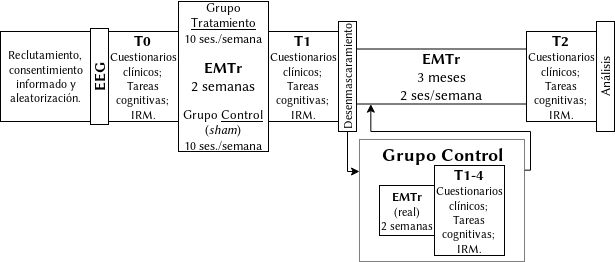
\includegraphics[width=\textwidth]{Des1}
    \caption{Linea de curso del tratamiento clínico de EMTr}
    \label{fig:txTMS}
\end{figure}

El estudio consiste en 4 etapas principales (Figura \ref{fig:txTMS}):
\begin{enumerate}[start=0,left=\parindent,label=T\arabic*:]
    \item Filtro de pacientes y etapa basal;
    \item 2 semanas de tratamiento aleatorizado;
\end{enumerate}
\begin{enumerate}[left=\parindent,label=T-4:]
    \item 2 semanas de tratamiento real (grupo sham);
\end{enumerate}
\begin{enumerate}[start=2,left=\parindent,label=T\arabic*:]
    \item 3 meses de tratamiento de mantenimiento.
\end{enumerate}

\section{Instrumentos}
\subsection{Medidas de craving y recaída}
\begin{description}
    \item[CCQ-G] Cuestionario de Craving de la Cocaína, versión general (Cocaine Craving Questionnaire, General); escala que evalúa el deseo intenso hacia la droga de forma promedio en la última semana \parencite{Tiffany1993}.
    \item[CCQ-N] Cuestionario de Craving a la Cocaína, versión actual (Cocaine Craving Questionnaire, Now); escala que evalúa de forma presente el deseo intenso hacia la droga en el momento de aplicación \parencite{Tiffany1993}.
    \item[VAS] Escala Visual Análoga; escala visual análoga de \SI{100}{\milli\meter} utilizada para representar el \textit{craving} en el momento.
    \item[Línea de tiempo restrospectiva] Calendario de consumo como herramiento para medir el \textbf{lapso} (por lo menos un evento de consumo con patrón diferente al basal) y \textbf{relapso} (evento de consumo con el mismo patrón que el consumo basal).
\end{description}
\subsection{Medida de impulsividad}
\begin{description}
    \item[BIS-11] Escala de impulsividad de Barratt 11 (Barratt Impulsivity Scale 11); escala clínica que evalúa multidimensionalmente el índice de impulsividad \parencite{H.Patton1995,SALVO2013}.
\end{description}
\begin{enumerate}[label=Subescala \arabic*., left= \parindent]
    \item Impulsividad atencional
    \item Impulsividad motora
    \item Impulsividad de no-planeación
\end{enumerate}

\section{Estimulación magnética transcraneal repetitiva (EMTr)}








